\section{Presentation}
\label{tree:pop:presentation}

\begin{figure}
	\centering
	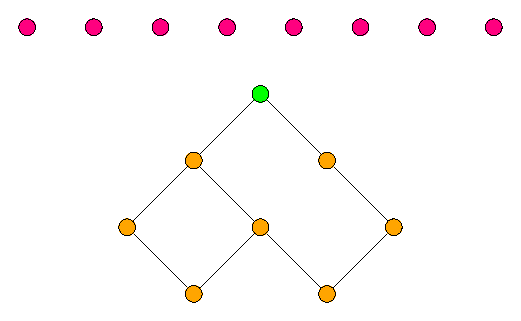
\includegraphics[width=0.6\textwidth]{fig/pop:diag}
	\caption{\label{fig:pop:diag} A partial order production problem.}
\end{figure}

The problem is the following,

Find a bijective relation between a Hasse diagram and an set of elements.

The input is thus composed of a partial order in form of a Hasse diagram and a set $A$ of elements (see \ref{fig:pop:diag}).

\cite{jcardin1} solves the Partial Order Production problem in 2 steps:

\begin{enumerate}
\item Produce a weak order $W$ from the partial order in O($n^3$);
\item Run a multiple selection algorithm on ($W$,$A$).
\end{enumerate}